

\tikzset{every picture/.style={line width=0.75pt}} %set default line width to 0.75pt        

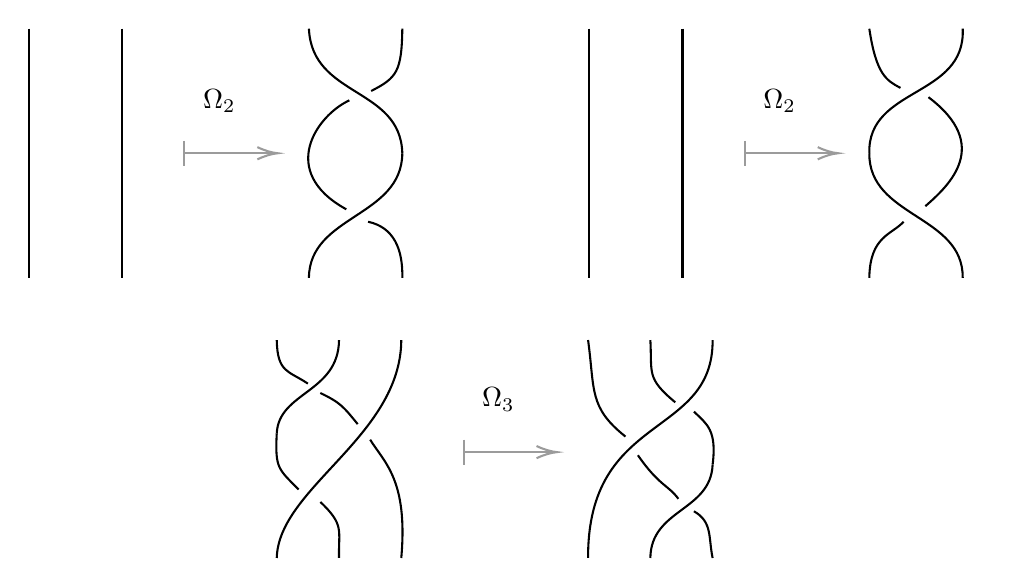
\begin{tikzpicture}[x=0.75pt,y=0.75pt,yscale=-1.5,xscale=1.5]
%uncomment if require: \path (0,300); %set diagram left start at 0, and has height of 300

%Straight Lines [id:da021068853778946184] 
\draw [color={rgb, 255:red, 155; green, 155; blue, 155 }  ,draw opacity=1 ]   (80,120) -- (108,120) ;
\draw [shift={(110,120)}, rotate = 180] [color={rgb, 255:red, 155; green, 155; blue, 155 }  ,draw opacity=1 ][line width=0.75]    (6.56,-1.97) .. controls (4.17,-0.84) and (1.99,-0.18) .. (0,0) .. controls (1.99,0.18) and (4.17,0.84) .. (6.56,1.97)   ;
%Straight Lines [id:da95151298393968] 
\draw [color={rgb, 255:red, 155; green, 155; blue, 155 }  ,draw opacity=1 ]   (80,116) -- (80,124) ;
%Straight Lines [id:da3105397663180821] 
\draw    (30,80) -- (30,160) ;
%Straight Lines [id:da41257341713042317] 
\draw    (60,80) -- (60,160) ;
%Curve Lines [id:da11900760040973013] 
\draw    (150,120) .. controls (149.8,140.6) and (120.2,139.8) .. (120,160) ;
%Curve Lines [id:da21344602026956538] 
\draw    (120,80) .. controls (121,102.2) and (149.4,98.6) .. (150,120) ;
%Curve Lines [id:da9689941604419631] 
\draw    (150,80) .. controls (149.8,93.8) and (148.2,95.8) .. (140,100) ;
%Curve Lines [id:da6960165665741206] 
\draw    (133,103) .. controls (122.6,107.8) and (109.8,125.8) .. (132,138) ;
%Curve Lines [id:da16812588273365814] 
\draw    (139,142) .. controls (147.4,143.8) and (150.2,151) .. (150,160) ;
%Straight Lines [id:da8993877656078348] 
\draw [color={rgb, 255:red, 155; green, 155; blue, 155 }  ,draw opacity=1 ]   (259.99,120) -- (287.99,120) ;
\draw [shift={(289.99,120)}, rotate = 180] [color={rgb, 255:red, 155; green, 155; blue, 155 }  ,draw opacity=1 ][line width=0.75]    (6.56,-1.97) .. controls (4.17,-0.84) and (1.99,-0.18) .. (0,0) .. controls (1.99,0.18) and (4.17,0.84) .. (6.56,1.97)   ;
%Straight Lines [id:da3147593233270113] 
\draw [color={rgb, 255:red, 155; green, 155; blue, 155 }  ,draw opacity=1 ]   (259.99,116) -- (259.99,124) ;
%Straight Lines [id:da36120199173040735] 
\draw    (209.99,80) -- (209.99,160) ;
%Straight Lines [id:da767115805534779] 
\draw    (239.99,80) -- (239.99,160) ;
%Curve Lines [id:da44641148036727185] 
\draw    (300,120) .. controls (299.8,140.6) and (330.2,139.8) .. (330,160) ;
%Curve Lines [id:da6320743672082285] 
\draw    (330,80) .. controls (331,102.2) and (299.4,98.6) .. (300,120) ;
%Curve Lines [id:da6313849027023718] 
\draw    (311,142) .. controls (307.2,146.2) and (300.2,146.6) .. (300,160) ;
%Curve Lines [id:da0589500737742894] 
\draw    (319,102) .. controls (339.4,117.4) and (325.8,130.2) .. (318,137) ;
%Curve Lines [id:da7255177605237971] 
\draw    (310,99) .. controls (305.4,96.6) and (302.2,94.6) .. (300,80) ;
%Curve Lines [id:da23638349304952366] 
\draw    (149.67,180) .. controls (149.47,211) and (110.27,227.4) .. (109.67,250) ;
%Curve Lines [id:da8983550529947678] 
\draw    (129.67,180) .. controls (129.47,197) and (110.27,196.6) .. (109.67,210) ;
%Curve Lines [id:da5344052460604444] 
\draw    (109.67,210) .. controls (109.07,221.4) and (110.27,221.4) .. (116.67,228) ;
%Curve Lines [id:da9058141972471662] 
\draw    (129.67,250) .. controls (129.47,241) and (131.47,239.4) .. (123.67,232) ;
%Curve Lines [id:da1999229819183379] 
\draw    (109.67,180) .. controls (109.87,190.6) and (113.47,189.8) .. (119.67,194) ;
%Curve Lines [id:da5382611206991912] 
\draw    (123.67,197) .. controls (130.27,200.2) and (131.07,201.4) .. (135.67,207) ;
%Curve Lines [id:da9383909926867282] 
\draw    (139.67,212) .. controls (144.27,219.4) and (151.87,225) .. (149.67,250) ;
%Straight Lines [id:da9655390534837395] 
\draw [color={rgb, 255:red, 155; green, 155; blue, 155 }  ,draw opacity=1 ]   (169.67,216) -- (197.67,216) ;
\draw [shift={(199.67,216)}, rotate = 180] [color={rgb, 255:red, 155; green, 155; blue, 155 }  ,draw opacity=1 ][line width=0.75]    (6.56,-1.97) .. controls (4.17,-0.84) and (1.99,-0.18) .. (0,0) .. controls (1.99,0.18) and (4.17,0.84) .. (6.56,1.97)   ;
%Straight Lines [id:da030621442854791958] 
\draw [color={rgb, 255:red, 155; green, 155; blue, 155 }  ,draw opacity=1 ]   (169.67,212) -- (169.67,220) ;
%Curve Lines [id:da5794729440142999] 
\draw    (249.67,180) .. controls (249.87,211.8) and (209.47,203) .. (209.67,250) ;
%Curve Lines [id:da10826159713872396] 
\draw    (229.67,180) .. controls (230.27,190.6) and (228.27,192.2) .. (237.67,200) ;
%Curve Lines [id:da991680044584273] 
\draw    (229.67,250) .. controls (229.87,234.2) and (249.07,235) .. (249.67,220) ;
%Curve Lines [id:da7350174882368962] 
\draw    (243.67,203) .. controls (247.87,207) and (251.07,209) .. (249.67,220) ;
%Curve Lines [id:da9744338524826922] 
\draw    (209.67,180) .. controls (211.87,196.2) and (209.87,201.6) .. (221.67,211) ;
%Curve Lines [id:da1740724973590062] 
\draw    (243.67,235) .. controls (249.67,238.4) and (248.27,243.4) .. (249.67,250) ;
%Curve Lines [id:da3320368868474375] 
\draw    (225.67,217) .. controls (232.47,226.8) and (235.47,226.6) .. (238.67,231) ;

% Text Node
\draw (85,98.4) node [anchor=north west][inner sep=0.75pt]    {$\Omega _{2}$};
% Text Node
\draw (264.99,98.4) node [anchor=north west][inner sep=0.75pt]    {$\Omega _{2}$};
% Text Node
\draw (174.67,194.4) node [anchor=north west][inner sep=0.75pt]    {$\Omega _{3}$};


\end{tikzpicture}